\documentclass[tikz,border=8pt]{standalone}
% Shared look for every TikZ diagram. Load with \input{../../tools/tikz-style.tex}
\usepackage[T1]{fontenc}
\usepackage{lmodern}
\renewcommand{\sfdefault}{lmr}  % diagrams use the same serif as the text
\usetikzlibrary{arrows.meta, positioning, shapes.geometric, calc, fit, backgrounds}
\definecolor{cblue}{HTML}{4C78A8}
\definecolor{corange}{HTML}{F58518}
\definecolor{cgreen}{HTML}{54A24B}
\definecolor{cred}{HTML}{E45756}
\definecolor{cpurple}{HTML}{B279A2}
\definecolor{cgrey}{HTML}{6B6B6B}
\tikzset{
  every picture/.style={font=\sffamily, line width=1.2pt},
  box/.style={draw=#1, fill=#1!12, rounded corners=4pt, align=center, inner sep=7pt, minimum height=1.1cm},
  box/.default=cgrey,
  arrow/.style={-{Stealth[length=3mm]}, draw=cgrey, line width=1.4pt},
  title/.style={font=\sffamily\bfseries\Large},
  note/.style={font=\sffamily\small, text=cgrey, align=center},
}
\AtBeginDocument{\hyphenpenalty=10000 \exhyphenpenalty=10000}

\newcommand{\cell}[4]{\node[draw=cgrey, line width=0.8pt, minimum size=0.95cm, fill=#4, font=\sffamily\large] at ({#1},{#2}) {#3};}
\begin{document}
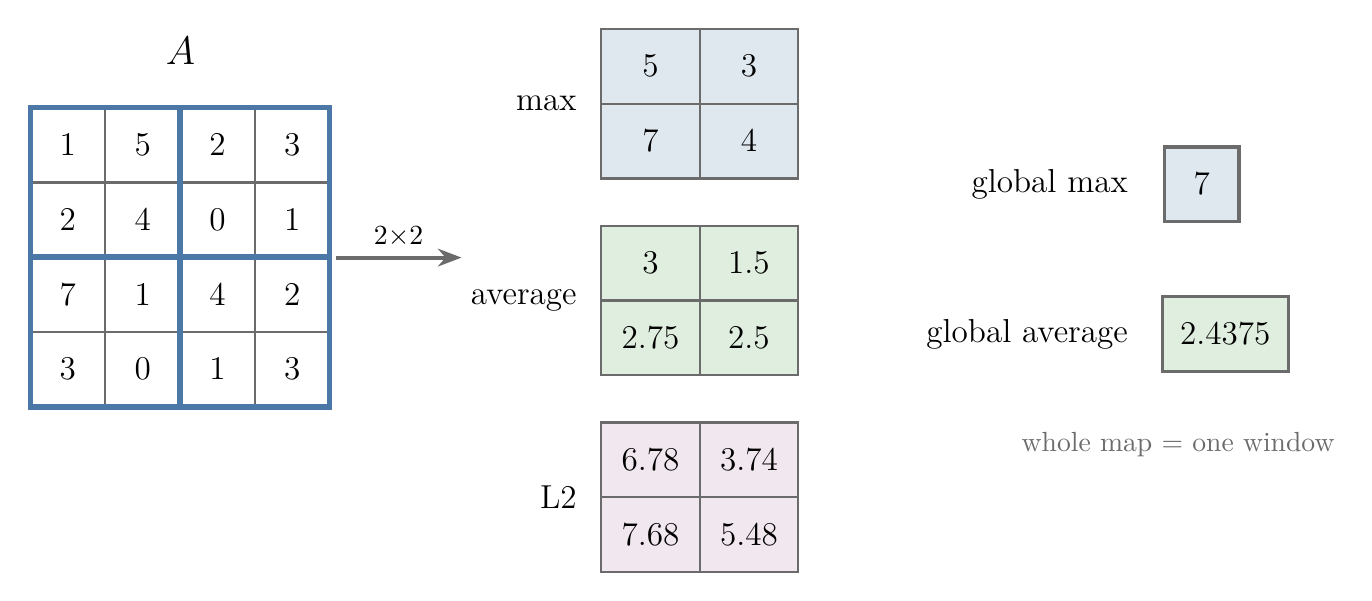
\begin{tikzpicture}
  \node[title] at (1.43,1.2) {$A$};
  \foreach \v [count=\i from 0] in {1,5,2,3,2,4,0,1,7,1,4,2,3,0,1,3}{
    \pgfmathtruncatemacro{\r}{\i/4}\pgfmathtruncatemacro{\c}{mod(\i,4)}
    \cell{\c*0.95}{-\r*0.95}{\v}{white}}
  \foreach \x/\y in {0/0, 1.9/0, 0/-1.9, 1.9/-1.9} \draw[cblue, line width=2pt] (\x-0.475,\y+0.475) rectangle ++(1.9,-1.9);
  % three window summaries
  \foreach \name/\vals/\col/\yy in {max/{5,3,7,4}/cblue/1.0, average/{3,1.5,2.75,2.5}/cgreen/-1.5, L2/{6.78,3.74,7.68,5.48}/cpurple/-4.0}{
    \node[font=\sffamily\large, anchor=east] at (6.6,\yy-0.47) {\name};
    \foreach \v [count=\i from 0] in \vals {
      \pgfmathtruncatemacro{\r}{\i/2}\pgfmathtruncatemacro{\c}{mod(\i,2)}
      \node[draw=cgrey, line width=0.8pt, minimum width=1.25cm, minimum height=0.95cm, fill=\col!18, font=\sffamily\large] at (7.4+\c*1.25, \yy-\r*0.95) {\v};}
  }
  \draw[arrow] (3.4,-1.43) -- (5.0,-1.43) node[midway, above] {2$\times$2};
  % global
  \node[font=\sffamily\large, anchor=east] at (13.6,-0.5) {global max};
  \node[draw=cgrey, minimum size=0.95cm, fill=cblue!18, font=\sffamily\large] at (14.4,-0.5) {7};
  \node[font=\sffamily\large, anchor=east] at (13.6,-2.4) {global average};
  \node[draw=cgrey, minimum width=1.6cm, minimum height=0.95cm, fill=cgreen!18, font=\sffamily\large] at (14.7,-2.4) {2.4375};
  \node[note, font=\sffamily\normalsize] at (14.1,-3.8) {whole map = one window};
\end{tikzpicture}
\end{document}
